\chapter{Establishing secure connections over insecure
channels}\label{12-Establishing-secure-co}

We've now compiled all the tools that are needed for the basic goal of
cryptography (which is still being subverted quite often) allowing Alice
and Bob to exchange messages assuring their integrity and
confidentiality over a channel that is observed or controlled by an
adversary. Our tools for achieving this goal are:

\begin{itemize}
\item
  Public key (aka asymmetric) encryption schemes.
\item
  Public key (aka asymmetric) digital signatures schemes.
\item
  Private key (aka symmetric) encryption schemes - block ciphers and
  stream ciphers.
\item
  Private key (aka symmetric) message authentication codes and
  pseudorandom functions.
\item
  Hash functions that are used both as ways to compress messages for
  authentication as well as key derivation and other tasks.
\end{itemize}

The notions of security we require from these building blocks can vary
as well. For encryption schemes we talk about CPA (chosen plaintext
attack) and CCA (chosen ciphertext attacks), for hash functions we talk
about collision-resistance, being used (combined with keys) as
pseudorandom functions, and then sometimes we simply model those as
random oracles. Also, all of those tools require access to a source of
randomness, and here we use hash functions as well for entropy
extraction.

\section{Cryptography's obsession with
adjectives.}\label{12-Cryptographys-obsessio}

As we learn more and more cryptography we see more and more adjectives,
every notion seems to have modifiers such as ``non-malleable'',
``leakage-resilient'', ``identity based'', ``concurrently secure'',
``adaptive'', ``non-interactive'', etc.. etc\ldots{} . Indeed, this
motivated a parody web page of an
\href{https://cseweb.ucsd.edu/~mihir/crypto-topic-generator.html}{automatic
crypto paper title generator}. Unlike algorithms, where typically there
are straightforward \emph{quantitative} tradeoffs (e.g., faster is
better), in cryptography there are many \emph{qualitative} ways
protocols can vary based on the assumptions they operate under and the
notions of security they provide.

In particular, the following issues arise when considering the task of
securely transmitting information between two parties Alice and Bob:

\begin{itemize}
\item
  \textbf{Infrastructure/setup assumptions:} What kind of setup can
  Alice and Bob rely upon? For example in the TLS protocol, typically
  Alice is a website and Bob is user; Using the infrastructure of
  certificate authorities, Bob has a trusted way to obtain Alice's
  \emph{public signature key}, while Alice doesn't know anything about
  Bob. But there are many other variants as well. Alice and Bob could
  share a (low entropy) \emph{password}. One of them might have some
  hardware token, or they might have a secure out of band channel (e.g.,
  text messages) to transmit a short amount of information. There are
  even variants where the parties authenticate by something they
  \emph{know}, with one recent example being the notion of \emph{witness
  encryption} (Garg, Gentry, Sahai, and Waters) where one can encrypt
  information in a ``digital time capsule'' to be opened by anyone who,
  for example, finds a proof of the Riemann hypothesis.
\item
  \textbf{Adversary access:} What kind of attacks do we need to protect
  against. The simplest setting is a \emph{passive} eavesdropping
  adversary (often called ``Eve'') but we sometimes consider an
  \emph{active person-in-the-middle} attacks (sometimes called
  ``Mallory''). We sometimes consider notions of \emph{graceful
  recovery}. For example, if the adversary manages to hack into one of
  the parties then it can clearly read their communications from that
  time onwards, but we would want their past communication to be
  protected (a notion known as \emph{forward secrecy}). If we rely on
  trusted infrastructure such as certificate authorities, we could ask
  what happens if the adversary breaks into those. Sometimes we rely on
  the security of several entities or secrets, and we want to consider
  adversaries that control \emph{some} but not \emph{all} of them, a
  notion known as \emph{threshold cryptography}. While we typically
  assume that information is either fully secret or fully public, we
  sometimes want to model \emph{side channel attacks} where the
  adversary can learn \emph{partial information} about the secret, this
  is known as \emph{leakage-resistant cryptography}.
\item
  \textbf{Interaction:} Do Alice and Bob get to interact and relay
  several messages back and forth or is it a ``one shot'' protocol? You
  may think that this is merely a question about efficiency but it turns
  out to be crucial for some applications. Sometimes Alice and Bob might
  not be two parties separated in space but the same party separated in
  time. That is, Alice wishes to send a message to her future self by
  storing an encrypted and authenticated version of it on some media. In
  this case, absent a time machine, back and forth interaction between
  the two parties is obviously impossible.
\item
  \textbf{Security goal:} The security goals of a protocol are usually
  stated in the negative- what does it mean for an adversary to
  \emph{win} the security game. We typically want the adversary to learn
  absolutely no information about the secret beyond what she obviously
  can. For example, if we use a shared password chosen out of \(t\)
  possibilities, then we might need to allow the adversary \(1/t\)
  success probability, but we wouldn't want her to get anything beyond
  \(1/t+negl(n)\). In some settings, the adversary can obviously
  completely disconnect the communication channel between Alice and Bob,
  but we want her to be essentially limited to either dropping
  communication completely or letting it go by unmolested, and not have
  the ability to modify communication without detection. Then in some
  settings, such as in the case of steganography and anonymous routing,
  we would want the adversary not to find out even the fact that a
  conversation had taken place.
\end{itemize}

\section{Basic Key Exchange protocol}\label{12-Basic-Key-Exchange-pro}

The basic primitive for secure communication is a \emph{key exchange}
protocol, whose goal is to have Alice and Bob share a common random
secret key \(k\in\{0,1\}^n\). Once this is done, they can use a CCA
secure / authenticated private-key encryption to communicate with
confidentiality and integrity.

The canonical example of a basic key exchange protocol is the
\emph{Diffie Hellman} protocol. It uses as public parameters a group
\(\mathbb{G}\) with generator \(g\), and then follows the following
steps:

\begin{enumerate}
\def\labelenumi{\arabic{enumi}.}
\item
  Alice picks random \(a\leftarrow_R\{0,\ldots,|\mathbb{G}|-1\}\) and
  sends \(A=g^a\).
\item
  Bob picks random \(b\leftarrow_R \{0,\ldots,|\mathbb{G}|-1\}\) and
  sends \(B=g^b\).
\item
  They both set their key as \(k=H(g^{ab})\) (which Alice computes as
  \(B^a\) and Bob computes as \(A^b\)), where \(H\) is some hash
  function.
\end{enumerate}

Another variant is using an arbitrary public key encryption scheme such
as RSA:

\begin{enumerate}
\def\labelenumi{\arabic{enumi}.}
\item
  Alice generates keys \((d,e)\) and sends \(e\) to Bob.
\item
  Bob picks random \(k \leftarrow_R\{0,1\}^m\) and sends \(E_e(k)\) to
  Alice.
\item
  They both set their key to \(k\) (which Alice computes by decrypting
  Bob's ciphertext)
\end{enumerate}

Under plausible assumptions, it can be shown that these protocols secure
against a \emph{passive} eavesdropping adversary Eve. The notion of
security here means that, similar to encryption, if after observing the
transcript Eve receives with probability \(1/2\) the value of \(k\) and
with probability \(1/2\) a random string \(k'\gets\{0,1\}^n\), then her
probability of guessing which is the case would be at most
\(1/2+negl(n)\) (where \(n\) can be thought of as \(\log |\mathbb{G}|\)
or some other parameter related to the length of bit representation of
members in the group).

\section{Authenticated key exchange}\label{12-Authenticated-key-exch}

The main issue with this key exchange protocol is of course that
adversaries often are \emph{not} passive. In particular, an active Eve
could agree on her own key with Alice and Bob separately and then be
able to see and modify all future communication. She might also be able
to create weird (with some potential security implications) correlations
by, say, modifying the message \(A\) to be \(A^2\) etc..

For this reason, in actual applications we typically use
\emph{authenticated} key exchange. The notion of authentication used
depends on what we can assume on the setup assumptions. A standard
assumption is that Alice has some public keys but Bob doesn't. The
justification for this assumption is that Alice might be a server, which
has the capabilities to generate a private/public key pair, disseminate
the public key (e.g., using a certificate authority) and maintain the
private key in a secure storage. In contrast, if Bob is an individual
user, then it might not have access to a secure storage to maintain a
private key (since personal devices can often are hacked). Moreover,
Alice might not care about Bob's identity. For example, if Alice is
nytimes.com and Bob is a reader, then Bob wants to know that the news he
reads really came from the \emph{New York Times}, but Alice is equally
happy to engage in communication with any reader. In other cases, such
as gmail.com, after an initial secure connection is setup, Bob can
authenticate himself to Alice as a registered user (by sending his login
information or sending a ``cookie'' stored from a past interaction).

It is possible to obtain a secure channel under these assumptions, but
one needs to be careful. Indeed, the standard protocol for securing the
web: the \href{https://goo.gl/md9Bsa}{transport Layer Security (TLS)
protocol} (and its predecessor SSL) has gone through six revisions
(including a name change from SSL to TLS) largely because of security
concerns. We now illustrate one of those attacks.

\subsection{Bleichenbacher's attack on RSA PKCS V1.5 and SSL
V3.0}\label{12-Bleichenbachers-attack}

If you have a public key, a natural approach is to take the
encryption-based protocol and simply skip the first step since Bob
already knows the public key \(e\) of Alice. This is basically what
happened in the SSL V3.0 protocol. However, as was
\href{http://archiv.infsec.ethz.ch/education/fs08/secsem/bleichenbacher98.pdf}{shown
by Bleichenbacher in 1998}, it turns out this is susceptible to the
following attack:

\begin{itemize}
\item
  The adversary listens in on a conversation, and in particular observes
  \(c=E_e(k)\) where \(k\) is the private key.
\item
  The adversary then starts many connections with the server with
  ciphertexts related to \(c\), and observes whether they succeed or
  fail (and in what way they fail, if they do). It turns out that based
  on this information, the adversary would be able to recover the key
  \(k\).
\end{itemize}

Specifically, the version of RSA (known as PKCS #V1.5) used in the SSL
V3.0 protocol requires the value \(x\) to have a particular format, with
the top two bytes having a certain form. If in the course of the
protocol, a server decrypts \(y\) and gets a value \(x\) not of this
form then it would send an error message and halt the connection. While
the designers of SSL V3.0 might not have thought of it that way, this
amounts to saying that an SSL V3.0 server supplies to any party an
oracle that on input \(y\) outputs \(1\) iff \(y^{d} \pmod{m}\) has this
form, where \(d = e^{-1} \pmod|\Z^*_m|\) is the secret decryption key.
It turned out that one can use such an oracle to invert the RSA
function. For a result of a similar flavor, see the (1/2 page) proof of
Theorem 11.31 (page 418) in KL, where they show that an oracle that
given \(y\) outputs the least significant bit of \(y^d \pmod{m}\) allows
to invert the RSA function.\footnote{The first attack of this flavor was
  given in the 1982 paper of Goldwasser, Micali, and Tong.
  Interestingly, this notion of ``hardcore bits'' has been used for both
  practical \emph{attacks} against cryptosystems as well as theoretical
  (and sometimes practical) \emph{constructions} of other cryptosystems.}

For this reason, new versions of the SSL used a different variant of RSA
known as PKCS #1 V2.0 which satisfies (under assumptions) \emph{chosen
ciphertext security (CCA)} and in particular such oracles cannot be used
to break the encryption. Nonetheless, there are still some
implementation issues that allowed to perform some attacks, specifically
\href{http://archiv.infsec.ethz.ch/education/fs08/secsem/Manger01.pdf}{Manger}
showed that depending on PKCS #1 V2.0 is implemented, it might be
possible to still launch an attack. The main reason is that the
specification states several conditions under which decryption box is
supposed to return ``error''. The proof of CCA security crucially relies
on the attacker not being able to distinguish which condition caused the
error message. However, some implementations could still leak this
information, for example by checking these conditions one by one, and so
returning ``error'' quicker when the earlier conditions hold. See
discussion in Katz-Lindell (3rd ed) 12.5.4.

\section{Chosen ciphertext attack security for public key
cryptography}\label{12-Chosen-ciphertext-atta}

The concept of chosen ciphertext attack security makes perfect sense for
\emph{public key} encryption as well. It is defined in the same way as
it was in the private key setting:

\hypertarget{CCSpubdef}{}
\begin{definition}[CCA secure public key encryption] \label[definition]{CCSpubdef}

A public key encryption scheme \((G,E,D)\) is \emph{chosen ciphertext
attack (CCA) secure} if every efficient Mallory wins in the following
game with probability at most \(1/2+ negl(n)\):

\begin{itemize}
\item
  The keys \((e,d)\) are generated via \(G(1^n)\), and Mallory gets the
  public encryption key \(e\) and \(1^n\).
\item
  For \(poly(n)\) rounds, Mallory gets access to the function
  \(c \mapsto D_d(c)\). (She doesn't need access to \(m \mapsto E_e(m)\)
  since she already knows \(e\).)
\item
  Mallory chooses a pair of messages \(\{ m_0,m_1 \}\), a secret \(b\)
  is chosen at random in \(\{0,1\}\), and Mallory gets
  \(c^* = E_e(m_b)\). (Note that she of course does \emph{not} get the
  randomness used to generate this challenge encryption.)
\item
  Mallory now gets another \(poly(n)\) rounds of access to the function
  \(c \mapsto D_d(c)\) except that she is not allowed to query \(c^*\).
\item
  Mallory outputs \(b'\) and \emph{wins} if \(b'=b\).
\end{itemize}

\end{definition}

In the private key setting, we achieved CCA security by combining a
CPA-secure private key encryption scheme with a message authenticating
code (MAC), where to CCA-encrypt a message \(m\), we first used the
CPA-secure scheme on \(m\) to obtain a ciphertext \(c\), and then added
an authentication tag \(\tau\) by signing \(c\) with the MAC. The
decryption algorithm first verified the MAC before decrypting the
ciphertext. In the public key setting, one might hope that we could
repeat the same construction using a CPA-secure \emph{public key}
encryption and replacing the MAC with \emph{digital signatures}.

\begin{pause} \label[pause]{12-Try-to-think-what-woul}

Try to think what would be such a construction, and whether there is a
fundamental obstacle to combining digital signatures and public key
encryption in the same way we combined MACs and private key encryption.

\end{pause}

Alas, as you may have realized, there is a fly in this ointment. In a
signature scheme (necessarily) it is the \emph{signing key} that is
\emph{secret}, and the \emph{verification key} that is \emph{public}.
But in a public key encryption, the \emph{encryption} key is
\emph{public}, and hence it makes no sense for it to use a secret
signing key. (It's not hard to see that if you reveal the secret signing
key then there is no point in using a signature scheme in the first
place.)

\paragraph{Why CCA security matters.} For the reasons above,
constructing CCA secure public key encryption is very challenging. But
is it worth the trouble? Do we really need this ``ultra conservative''
notion of security? The answer is \emph{yes}. Just as we argued for
\emph{private key} encryption, chosen ciphertext security is the notion
that gets us as close as possible to designing encryptions that fit the
metaphor of \emph{secure sealed envelopes}. Digital analogies will never
be a perfect imitation of physical ones, but such metaphors are what
people have in mind when designing cryptographic protocols, which is a
hard enough task even when we don't have to worry about the ability of
an adversary to reach inside a sealed envelope and XOR the contents of
the note written there with some arbitrary string. Indeed, several
practical attacks, including Bleichenbacher's attack above, exploited
exactly this gap between the physical metaphor and the digital
realization. For more on this, please see
\href{http://www.shoup.net/papers/expo.pdf}{Victor Shoup's survey} where
he also describes the Cramer-Shoup encryption scheme which was the first
practical public key system to be shown CCA secure without resorting to
the random oracle heuristic. (The first definition of CCA security, as
well as the first polynomial-time construction, was given in a seminal
1991 work of Dolev, Dwork and Naor.)

\section{CCA secure public key encryption in the Random Oracle
Model}\label{12-CCA-secure-public-key-}

We now show how to convert any CPA-secure public key encryption scheme
to a CCA-secure scheme in the random oracle model (this construction is
taken from Fujisaki and Okamoto, CRYPTO 99). In the homework, you will
see a somewhat simpler direct construction of a CCA secure scheme from a
\emph{trapdoor permutation}, a variant of which is known as OAEP (which
has better ciphertext expansion) has been standardized as PKCS #1 V2.0
and is used in several protocols. The advantage of a generic
construction is that it can be instantiated not just with the RSA and
Rabin schemes, but also directly with Diffie-Hellman and Lattice based
schemes (though there are direct and more efficient variants for these
as well).

\begin{quote} \label[quote]{12-CCA-ROM-ENC-SchemeIngr}

\textbf{CCA-ROM-ENC Scheme:}

\begin{itemize}
\item
  \textbf{Ingredients:} A CPA-secure public key encryption scheme
  \((G',E',D')\) and three hash functions
  \(H,H',H'':\{0,1\}^*\rightarrow\{0,1\}^n\) (which we model as
  independent random oracles\footnote{Recall that it's easy to obtain
    two independent random oracles \(H,H'\) from a single oracle
    \(H''\), for example by letting \(H(x)=H''(0\|x)\) and
    \(H'(x)=H''(1\|x)\).}).
\item
  \emph{Notes:} We assume that \(E'\) takes \(n\) bit messages (since
  CPA security is preserved under concatenation, a one-bit scheme can be
  transformed into such a scheme). Since \(E'\) is (necessarily)
  randomized, we denote by \(E'(x;s)\) the encryption of the message
  \(x\) using the randomness \(s\). We assume that the number of bits of
  randomness \(E'\) uses is \(n\). (Otherwise we can modify the scheme
  to use \(n\) bits using a pseudorandom generator, or modify the
  co-domain of \(H\) to be the space of random choices for \(E'\).)
\item
  \textbf{Key generation:} We generate keys \((e,d)=G'(1^n)\) for the
  underlying encryption scheme.
\item
  \textbf{Encryption:} To encrypt a message \(m\in\{0,1\}^\ell\), we
  select \(r \leftarrow_R \{0,1\}^n\), and output
\end{itemize}

\begin{equation*}
E_e(m) = E'_e(r ; H(m\|r)) \| H''(r) \oplus m \| H'(m \| r)
\end{equation*}

recall that \(E'_e(r ; s)\) denotes the encryption of the message \(r\)
using randomness \(s\).

\begin{itemize}
\tightlist
\item
  \textbf{Decryption:} To decrypt a ciphertext \(c\|y \| h\) first let
  \(r=D'_d(c)\), then compute \(m=H''(r) \oplus y\). Finally check that
  \(c= E'_e(m ; H(m\|r))\) and \(h=H'(m\|r)\). If either check fails we
  output \texttt{error}; otherwise we output \(m\).
\end{itemize}

\end{quote}

\hypertarget{CCAPKCthm}{}
\begin{theorem}[CCA security from random oracles] \label[theorem]{CCAPKCthm}

The above CCA-ROM-ENC scheme is CCA secure.

\end{theorem}

\begin{proof} \label[proof]{12-Let-A-be-a-polynomial-}

Let \(A\) be a polynomial-time adversary that wins the ``CCA Game'' with
respect to the scheme \((G,E,D)\) with probability \(1/2 + \epsilon\).
We will show (Claim 1) that there is an adversary \(\tilde{A}\) that can
win in this game with probability \(1/2 + \epsilon - negl(n)\)
\emph{without using the decryption box}. We will then show (Claim 2)
that this implies that \(A'\) can win the \emph{CPA game} with respect
to the scheme \((G',E',D')\) with probability
\(1/2 + \Omega(\epsilon)\). We start by establishing the first claim:

\textbf{Claim 1:} Under the above assumptions, there exists a
polynomial-time adversary \(\tilde{A}\) that wins the CCA game with
respect to the scheme \((G,E,D)\) without making any queries to the
decryption box.

\textbf{Proof of Claim 1:} The adversary \(\tilde{A}\) will simulate
\(A\), keeping track of all of \(A\)'s queries to its decryption and
random oracles. Whenever \(A\) makes a query \(c\|y\|h\) to the
decryption oracle, then \(\tilde{A}\) will respond to it using the
following ``fake'' decryption box \(\tilde{D}\): check whether \(h\) was
returned before from the random oracle \(H'\) as a response to a query
\(m\|r\) by \(A\). If this is the case, then \(\tilde{A}\) will check if
\(c = E'_e(r;H(m\|r))\) and \(y= H''(r) \oplus m\). If so, then it will
return \(m\), otherwise it will return \texttt{error}. Note that
\(\tilde{D}(c\|y\|h)\) is computed without any knowledge of the secret
key \(d\).

We claim that the probability that \(\tilde{A}\) will return an answer
that differs from the true decryption box is negligible. Indeed, for
each particular query \(c\|y\|h\), first observe that if
\(\tilde{D}(c\|y\|h)\) is not \texttt{error} then
\(\tilde{D}(c\|y\|h) = D_d(c\|y\|h)\). Indeed, in this case it holds
that \(c=E'_e(m;H(m\|r))\), \(y=H'(r) \oplus m\) and \(h=H'(m\|r)\).
Hence this is a properly formatted encryption of \(m\), on which the
true decryption box will return \(m\) as well.

So the only way that \(D\) and \(\tilde{D}\) differ is if
\(D_d(c\|y\|h)=m\) but \(\tilde{D}(c\|y\|h)\) returns \texttt{error}.
For this it must be the case that for \(r=D'_d(c)\), \(h=H'(m\|r)\) but
\(m\|r\) was \emph{not} queried before by \(A\). There are two options:
either \(m\|r\) was not queried at all, but then by the ``lazy
evaluation'' paradigm, the value \(H'(m\|r)\) is chosen uniformly in
\(\{0,1\}^n\) independently of \(h\), and the probability that it equals
\(h\) is \(2^{-n}\). The other option is that \(m\|r\) was queried by
not by the adversary. The only other party that can make queries to the
oracle in the CCA game is the challenger, and it only makes a single
query to \(H'\) when producing the challenge ciphertext
\(C^* = c^*\|y^*\|h^*\) with \(h^* = H'(m^*\|r^*)\). Now the adversary
is not allowed to make the query \(C^*\) so in this case the query must
have the form \(c\|y\|h^*\) where \(c\|y \neq c^*\|y^*\). But the only
way that \(D_d(c\|y\|h^*)\) returns a value other than \texttt{error} is
if for \(r=D'_d(c)\) and \(m = y \oplus H''(r)\), \(c=E_e(r;H(m\|r))\)
and \(h^* = H'(m\|r)\). Since the probability of a collision in \(H'\)
is negligible, this can only happen if \(m\|r = m^*\|r^*\), but in this
case it will hold that \(c=c^*\) and \(y=y^*\), contradicting the fact
that the ciphertext must differ from \(C^*\). \textbf{QED (Claim 1)}

\textbf{Claim 2:} Under the above assumptions, there exists a
polynomial-time adversary \(A'\) that wins the CPA game with respect to
the scheme \((G',E',D')\) with probability at least
\(1/2 + \epsilon/10\).

\textbf{Proof of Claim 2:}\\
\(A'\) runs the full CCA experiment with the adversary \(\tilde{A}\)
obtained from Claim 1, simulating the random oracles \(H,H',H''\) using
``lazy evaluation''. When the time comes and the adversary \(\tilde{A}\)
chooses two ciphertexts \(m_0,m_1\), then \(A'\) does the following:

\begin{enumerate}
\def\labelenumi{\arabic{enumi}.}
\item
  The adversary \(A'\) will choose \(r_0,r_1 \leftarrow_R \{0,1\}^n\),
  give them to its own challenger and get \(c^*\) which is either an
  encryption of \(r_{b^*}\) under \(E'_e\) for
  \(b^* \leftarrow_R \{0,1\}\). If the adversary \(\tilde{A}\) made in
  the past a query of the form \(r_b\) or \(m_b\|r_{b'}\) for
  \(b,b' \in \{0,1\}\) to one of the random oracles then we stop the
  experiment and declare failure. (Since \(r_0,r_1\) are random in
  \(\{0,1\}^n\) and \(\tilde{A}\) made only polynomially many queries,
  the probability of this happening is negligible).
\item
  The adversary \(A'\) will now give \(c^* \| y^* \| h^*\) with
  \(y^*,h^* \leftarrow_R \{0,1\}^n\) to \(\tilde{A}\) as the response to
  the challenge. (Note that this ciphertext does not involve neither
  \(m_0\) nor \(m_1\) in any way.)
\item
  Now if the adversary \(\tilde{A}\) makes a query of the form \(r_b\)
  or \(m\|r_b\) for \(b\in \{0,1\}\) to one of its oracles, then \(A'\)
  will output \(b\). Otherwise, it outputs a random output.
\end{enumerate}

Note that the adversary \(A'\) ignores the \emph{output} of
\(\tilde{A}\). It only cares about the queries that \(\tilde{A}\) makes.
Let's say that an ``\(r_b\) query is one that has \(r_b\) as a
postfix''. To finish the proof we make the following two claims:

\textbf{Claim 2.1:} The probability that \(\tilde{A}\) makes an
\(r_{1-b^*}\) query is negligible. \textbf{Proof:} This is because the
only value that \(\tilde{A}\) receives that depends on one of
\(r_0,r_1\) is \(c^*\) which is an encryption of \(r_{b^*}\). Hence
\(\tilde{A}\) never sees any value that depends on \(r_{1-b^*}\) and
since it is uniform in \(\{0,1\}^n\), the probability that \(\tilde{A}\)
makes a query with this postfix is negligible.

\textbf{Claim 2.2:} \(\tilde{A}\) will make an \(r_{b^*}\) query with
probability at least \(\epsilon/2\). \textbf{Proof:} Let
\(c^* = E'_e(r_{b^*} ; s^*)\) where \(s^*\) is the randomness used in
producing it. By the lazy evaluation paradigm, since no \(r_{b^*}\)
query was made up to that point, the distribution would be identical if
we defined \(H(m_b\|r_{b^*))=s^*\), defined
\(H''(r_{b^*)) = y^* \oplus m_b\) and define \(h^* = H'(m_b\|r_{b^*))\).
Hence the distribution of the ciphertext is identical to how it is
distributed in the actual CCA game. Now, since \(\tilde{A}\) wins the
CCA game with probability \(1/2 + \epsilon - negl(n)\), in this game it
must query \(H''\) at \(r_{b^*}\) with probability at least
\(\epsilon/2\). Indeed, conditioned on not querying \(H''\) at this
value, the string \(y^*\) is independent of the message \(m_0\), and the
adversary cannot win the game with probability more than \(1/2\).

Together Claims 2.1 and 2.2 imply that the adversary \(\tilde{A}\) makes
an \(r_{b^*}\) query with probability at least \(\epsilon/2\), and makes
an \(r_{1-b^*}\) query with negligible probability, hence our adversary
\(A'\) will output \(b^*\) with probability at least \(\epsilon/2\), and
with all but a negligible part of the remaining probability will guess
randomly, leading to an overall success in the CPA game of at least
\(1/2 + \epsilon/2\). \textbf{QED (Claim 2 and hence theorem)}

\end{proof}

\subsection{Defining secure authenticated key
exchange}\label{12-Defining-secure-authen}

The basic goal of secure communication is to set up a \emph{secure
channel} between two parties Alice and Bob. We want to do so over an
open network, where messages between Alice and Bob might be read,
modified, deleted, or added by the adversary. Moreover, we want Alice
and Bob to be sure that they are talking to one another rather than
other parties. This raises the question of what is identity and how is
it verified. Ultimately, if we want to use identities, then we need to
trust some authority that decides which party has which identity. This
is typically done via a \emph{certificate authority (CA)}. This is some
trusted authority, whose verification key \(v_{CA}\) is public and known
to all parties. Alice proves in some way to the CA that she is indeed
Alice, and then generates a pair \((s_{Alice},v_{Alice})\), and gets
from the CA the message \(\sigma_{Alice}\)=``The key \(v_{Alice}\)
belongs to Alice'' signed with \(s_{CA}\).\footnote{The registration
  process could be more subtle than that, and for example Alice might
  need to \emph{prove} to the CA that she does indeed know the
  corresponding secret key.} Now Alice can send
\((v_{Alice},\sigma_{Alice})\) to Bob to certify that the owner of this
public key is indeed Alice.

For example, in the web setting, certain
\href{https://en.wikipedia.org/wiki/Certificate_authority}{certificate
authorities} can certify that a certain public key is associated with a
certain website. If you go to a website using the \texttt{https}
protocol, you should see a ``lock'' symbol on your browser which will
give you details on the certificate. Often the certificate is a chain of
certificate. If I click on this lock symbol in my Chrome browser, I see
that the certificate that amazon.com's public key is some particular
string (corresponding to a 2048 RSA modulos and exponent) is signed by
the Symantec Certificate authority, whose own key is certified by
Verisign. My communication with Amazon is an example of a setting of
\emph{one sided authentication}. It is important for me to know that I
am truly talking to amazon.com, while Amazon is willing to talk to any
client. (Though of course once we establish a secure channel, I could
use it to login to my Amazon account.) Chapter 21 of Boneh Shoup
contains an in depth discussion of authenticated key exchange protocols,
see for example \cref{BSAKEfig}. Because the definition is so involved,
we will not go over the full formal definitions in this book, but I
recommend Boneh-Shoup for an in-depth treatment.

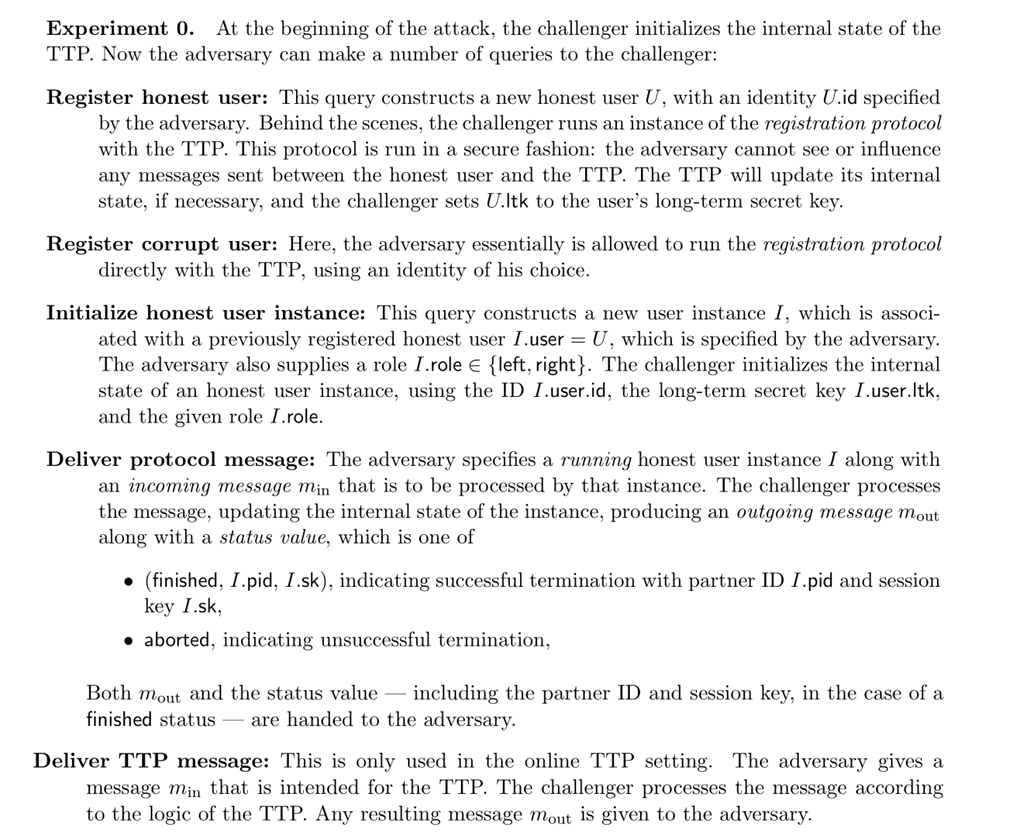
\includegraphics{../figure/AKEdef.png} the definitions of protocols AEK1
- AEK4.

\subsection{The compiler approach for authenticated key
exchange}\label{12-The-compiler-approach-}

There is a generic ``compiler'' approach to obtaining authenticated key
exchange protocols:

\begin{itemize}
\item
  Start with a protocol such as the basic Diffie-Hellman protocol that
  is only secure with respect to a \emph{passive eavesdropping}
  adversary.
\item
  Then \emph{compile} it into a protocol that is secure with respect to
  an active adversary using authentication tools such as digital
  signatures, message authentication codes, etc.., depending on what
  kind of setup you can assume and what properties you want to achieve.
\end{itemize}

This approach has the advantage of being modular in both the
construction and the analysis. However, direct constructions might be
more efficient. There are a great many potentially desirable properties
of key exchange protocols, and different protocols achieve different
subsets of these properties at different costs. The most common variant
of authenticated key exchange protocols is to use some version of the
Diffie-Hellman key exchange. If both parties have public signature keys,
then they can simply sign their messages and then that effectively rules
out an active attack, reducing active security to passive security
(though one needs to include identities in the signatures to ensure non
repeating of messages, see
\href{http://link.springer.com/article/10.1007\%2FBF00124891}{here}).

The most efficient variants of Diffie Hellman achieve authentication
implicitly, where the basic protocol remains the same (sending \(X=g^x\)
and \(Y=g^y\)) but the computation of the secret shared key involves
some authentication information. Of these protocols a particularly
efficient variant is the MQV protocol of Law, Menezes, Qu, Solinas and
Vanstone (which is based on similar principles as DSA signatures), and
its variant \href{https://eprint.iacr.org/2005/176.pdf}{HMQV} by
Krawczyk that has some improved security properties and analysis.

\section{Password authenticated key
exchange.}\label{12-Password-authenticated}

\paragraph{NOTE:} The following three parts are not yet written - we
will discuss them in class, but please at least skim the resources
pointed out below

PAKE is covered in Boneh-Shoup Chapter 21.11

\section{Client to client key exchange for secure text messaging - ZRTP,
OTR, TextSecure}\label{12-Client-to-client-key-e}

To be completed. See
\href{http://blog.cryptographyengineering.com/2013/03/here-come-encryption-apps.html}{Matthew
Green's blog} ,
\href{https://whispersystems.org/blog/advanced-ratcheting/}{text
secure}, \href{https://otr.cypherpunks.ca/Protocol-v3-4.0.0.html}{OTR}.

Security requirements: forward secrecy, deniability.

\section{Heartbleed and logjam attacks}\label{12-Heartbleed-and-logjam-}

\begin{itemize}
\item
  Vestiges of past crypto policies.
\item
  Importance of ``perfect forward secrecy''
\end{itemize}

\begin{marginfigure}
\centering
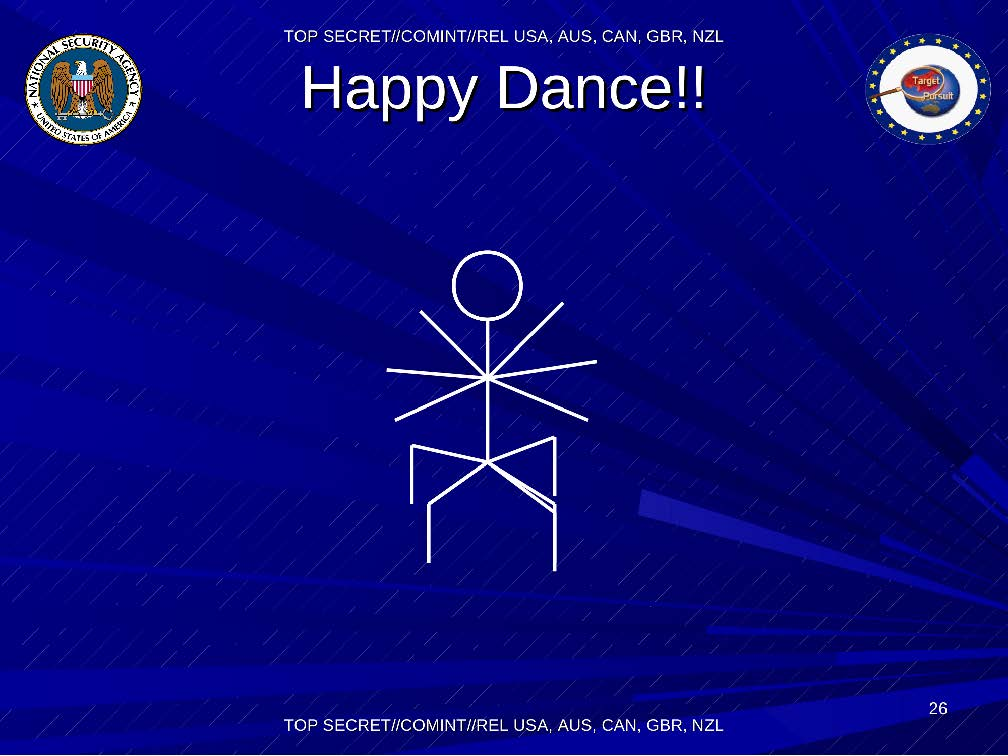
\includegraphics[width=\linewidth, height=1.5in, keepaspectratio]{../figure/NSA_Page_29.jpg}
\caption{How the NSA feels about breaking encrypted communication}
\label{tmplabelfig}
\end{marginfigure}
